\documentclass[../basicOrbitalDynamics.tex]{subfiles}
\graphicspath{{\subfix{../images/}}}
\begin{document}

Throughout this section, burns are assumed to be pseudo-impulsive. That is to say, they occur over an infinitesimal amount of distance and time. The $n$ vectors can change throughout the burn (and in fact, they do) with change in direction of velocity. It is assumed for ease of analysis that the spacecraft's thrust vector shifts to keep up with the $m$ vectors. It is important to remember that the $m$ vectors are based on velocity, not on position. That is to say, $\hat{m}_r$ does not necessarily point outward from the planet, but rather it points perpendicular to the velocity vector and in plane with the orbit. Only at the apses does $\hat{m}_v$ point perpendicular to the displacement from the planet. Similarly, only at the apses does $\hat{m}_r$ point radially outward from the planet.

\bigskip\bigskip
\subsection{Rocket Equation}

The rocket equation describes the relationship between the obtained change in velocity $\Delta{}v$ is related to the change in mass of a spacecraft.

\begin{figure}[H]
    \centering
    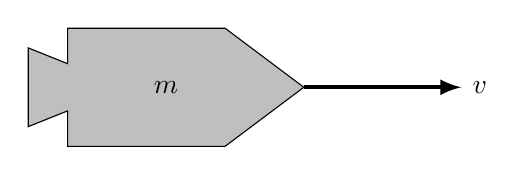
\begin{tikzpicture}[>=latex]
        \filldraw[lightgray, draw=black] (3.5,0)--(2.5,.75)--(0.5,.75)--(0.5,0.3)--(0,0.5)--(0,0)--(0,-0.5)--(0.5,-0.3)--(0.5,-.75)--(2.5,-.75)--cycle;
        \draw[ultra thick, ->] (3.5,0)--+(2,0) node[right] {$v$};
        %\draw[ultra thick, ->] (-1,0)--+(-2,0) node[left] {$v_e$};
        %\node[circle, fill=white, draw=gray] at (-1,0) {$m_e$};
        \node[] at (1.75,0) {$m$};
    \end{tikzpicture}

    \bigskip

    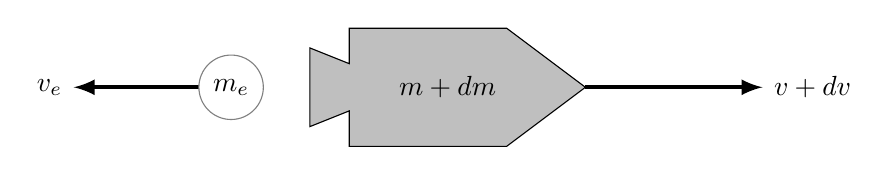
\begin{tikzpicture}[>=latex]
        \filldraw[lightgray, draw=black] (3.5,0)--(2.5,.75)--(0.5,.75)--(0.5,0.3)--(0,0.5)--(0,0)--(0,-0.5)--(0.5,-0.3)--(0.5,-.75)--(2.5,-.75)--cycle;
        \draw[ultra thick, ->] (3.5,0)--+(2.25,0) node[right] {$v+dv$};
        \draw[ultra thick, ->] (-1,0)--+(-2,0) node[left] {$v_e$};
        \node[circle, fill=white, draw=gray] at (-1,0) {$m_e$};
        \node[] at (1.75,0) {$m+dm$};
    \end{tikzpicture}

    \caption{A spacecraft with some exhaust exiting it}
\end{figure}

First, conservation of energy will be applied. For mass to be conserved, $m_e=-dm$.
\begin{align*}
    p_1                & =p_2                                                  \\
    \st{p}{rocket,1}  & =\st{p}{rocket,2}+\st{p}{exhaust}                   \\
    mv                 & =(m+dm)(v+dv)+m_e(v-v_e)                              \\
    mv                 & =(m+dm)(v+dv)-dm(v-v_e)                               \\
    mv                 & =mv+mdv+vdm+dmdv-vdm+v_edm                            \\
    \cancel{mv}        & =\cancel{mv}+mdv+\cancel{vdm}+dmdv-\cancel{vdm}+v_edm \\
    0                  & =mdv+dmdv+v_edm                                       \\
                       & \text{The second-order differential $dmdv$ vanishes}  \\
    0                  & =mdv+v_edm                                            \\
    -mdv               & =v_edm                                                \\
    dv                 & =\frac{-v_edm}{m}                                     \\
    \int_{v_1}^{v_2}dv & =-v_e\int_{m_1}^{m_2}\frac{1}{m}dm                    \\
    \Delta{}v          & =-v_e(\ln(m_2)-\ln(m_1))                              \\
    \Delta{}v          & =-v_e\ln(\frac{m_2}{m_1})                             \\
\end{align*}

\begin{equation}\label{Rocket Equation Ve}
    \Delta{}v=v_e\ln\left(\frac{m_1}{m_2}\right)
\end{equation}

This equation has another (equivalent) form. Because exhaust velocity can come in many different units, making it hard to compare between spacecraft. Instead of the exhaust velocity, a specific impulse $I_sp$ is defined. The specific impulse is the exhaust velocity divided by Earth's standard gravity at sea level. This allows the units to cancel out to seconds. $I_{sp}=\frac{v_e}{g_0}\rightarrow{}v_e=I_{sp}g_0$

\begin{equation}\label{Rocket Equation ISP}
    \Delta{}v=I_{sp}g_0\ln\left(\frac{m_1}{m_2}\right)
\end{equation}

Note that $\Delta v$ is not actually the change in velocity; a spacecraft can burn for a change in velocity of some arbitrary amount $\delta$ in one direction, then perform a burn of equal magnitude in a perpendicular direction. The magnitude of the change in velocity of the spacecraft is $\sqrt{2}\delta$, while the change in magnitude of velocity would depend on the initial velocity vector of the spacecraft. Instead, $\Delta v$ can be treated as a quantity that a spacecraft expends as it performs manuevers. For the rest of this chapter, the uppercase $\Delta V$ will be used to make this distinction, with the differential form $dV$ being used as well. Keep in mind that, while $dV$ and $\Delta V$ have units of velocity, they are \textit{not} necessarily equal to differential or absolute changes in the actual magnitude of velocity. When $dV$ is integrated, the integration bounds will be $V$- think of this as the currency which is being used, or a means of measuring fuel requirements for maneuvers.

\bigskip\bigskip
\subsection{Burns in the \texorpdfstring{$\hat{m}_r$}{Radial} Direction}\label{sec:Mr manuevers}

\begin{figure}[H]
    \centering
    \begin{tikzpicture}[>=latex]
        \def\vel{3}
        \def\dV{0.5}
        \def\velLong{\fpeval{sqrt(\vel^2+\dV^2)}}
        \def\dPhi{\fpeval{atan(\dV/\vel)}}
        \def\arcRad{1.5}
        \def\unMag{0.75}

        \draw[->] (0,0) -- +({deg(\dPhi)}:\velLong) node[midway,sloped,above] {$v'$};
        \draw[->] (0,0) -- +(\vel,0) node[midway,below] {$v$};
        \draw[->] (\vel,0) -- +(0,\dV) node[midway,right] {$dV$};
        \draw[] (\arcRad,0) arc (0:{deg(\dPhi)}:\arcRad) node[midway, right] {\tiny $d\phi$};

        \draw[densely dashed, -{Latex[open]}, gray, thick] (-1.5,0) -- +(90:\unMag) node[right] {$\hat{m}_r$};
        \draw[densely dashed, -{Latex[open]}, gray, thick] (-1.5,0) -- +(0:\unMag) node[right] {$\hat{m}_v$};
    \end{tikzpicture}
    \caption{Velocity change due to thrust in the $\hat{m}_r$ direction}\label{fig:dV Triangle Mr}
\end{figure}

It can be shown that $v'=v$.

\begin{align*}
    v'     & = \sqrt{v^2+dV^2}                                        \\
    (v')^2 & = v^2+dV^2                                               \\
    (v')^2 & = v^2+\cancelto{\text{smaller order differential}}{dV^2} \\
    (v')^2 & = v^2                                                    \\
    v'     & = v                                                      \\
\end{align*}

This proves that, when $dV$ is always perpendicular to the velocity vector, there is no change in magnitude of velocity. Because the magnitude of velocity is conserved, Equation \eqref{Specific Energy Physical} implies that specific energy is conserved. Equation \eqref{Specific Energy Geometric} shows that the semi-major axis is also unchanged due to the conservation of specific energy.

However, the flight path angle $\phi$ does change. Remember throughout this process that $v$ is constant.

\begin{align*}
    dV                     & =vd\phi                         \\
    d\phi                  & = \frac{dV}{v}                  \\
    \int_{\phi_1}^{\phi_2} & = \frac{1}{v}\int_{V_1}^{V_2}dV \\
    \Delta \phi            & = \frac{\Delta V}{v}            \\
\end{align*}

While the magnitude of velocity is not changed, its direction relative to the $u$ vectors (and any inertial base frame) is changed. Equation \eqref{Flight Path Angle} shows the relationship between $\phi$ and geometric parameters of the orbit.
$$\cos(\phi)=\sqrt{\frac{a^2(1-e^2)}{r(2a-r)}}$$

Because $a$ and $r$ are unchanged, $e$ must change. The precise change in $e$ can be investigated by solving for $e_2$, the eccentricity of the orbit post-burn.

\begin{align*}
    \sqrt{\frac{a^2(1-e_2^2)}{r(2a-r)}}                                   & =\cos(\phi+\Delta \phi)                                                                                                 \\
                                                                          & =\cos(\phi)\cos(\Delta \phi)-\sin(\phi)\sin(\Delta \phi)                                                                \\
                                                                          & =\cos(\phi)\cos(\Delta \phi)-\sqrt{1-\cos^2(\phi)}\sin(\Delta \phi)                                                     \\
                                                                          & =\sqrt{\frac{a^2(1-e^2)}{r(2a-r)}}\cos(\Delta \phi)-\sqrt{1-\frac{a^2(1-e^2)}{r(2a-r)}}\sin(\Delta \phi)                \\
    \sqrt{\frac{a^2(1-e_2^2)}{r(2a-r)}}/\sqrt{\frac{a^2(1-e^2)}{r(2a-r)}} & =\cos(\Delta \phi)-\frac{\sqrt{1-\frac{a^2(1-e^2)}{r(2a-r)}}}{\sqrt{\frac{a^2(1-e^2)}{r(2a-r)}}}\sin(\Delta \phi)       \\
    \sqrt{\frac{a^2(1-e_2^2)}{a^2(1-e^2)}}                                & =\cos(\Delta \phi)-\frac{\sqrt{\frac{r(2a-r)-a^2(1-e^2)}{r(2a-r)}}}{\sqrt{\frac{a^2(1-e^2)}{r(2a-r)}}}\sin(\Delta \phi) \\
    \sqrt{\frac{1-e_2^2}{1-e^2}}                                          & =\cos(\Delta \phi)-\sqrt{\frac{\frac{r(2a-r)-a^2(1-e^2)}{r(2a-r)}}{\frac{a^2(1-e^2)}{r(2a-r)}}}\sin(\Delta \phi)        \\
    \sqrt{\frac{1-e_2^2}{1-e^2}}                                          & =\cos(\Delta \phi)-\sqrt{\frac{r(2a-r)-a^2(1-e^2)}{a^2(1-e^2)}}\sin(\Delta \phi)                                        \\
    \sqrt{\frac{1-e_2^2}{1-e^2}}                                          & =\cos(\Delta \phi)-\sqrt{\frac{r(2a-r)}{a^2(1-e^2)}-1}\sin(\Delta \phi)                                                 \\
    \sqrt{\frac{1-e_2^2}{1-e^2}}                                          & =\cos(\Delta \phi)-\sqrt{1/\left(\sqrt{\frac{a^2(1-e^2)}{r(2a-r)}}\right)^2-1}\sin(\Delta \phi)                         \\
    \sqrt{\frac{1-e_2^2}{1-e^2}}                                          & =\cos(\Delta \phi)-\sqrt{\frac{1}{\cos^2(\phi)}-1}\sin(\Delta \phi)                                                     \\
    \sqrt{\frac{1-e_2^2}{1-e^2}}                                          & =\cos(\Delta \phi)-\sqrt{\sec^2(\phi)-1}\sin(\Delta \phi)                                                               \\
    \sqrt{\frac{1-e_2^2}{1-e^2}}                                          & =\cos(\Delta \phi)-\sqrt{\tan^2(\phi)}\sin(\Delta \phi)                                                                 \\
    \sqrt{\frac{1-e_2^2}{1-e^2}}                                          & =\cos(\Delta \phi)-\tan(\phi)\sin(\Delta \phi)                                                                          \\
    \frac{1-e_2^2}{1-e^2}                                                 & =(\cos(\Delta \phi)-\tan(\phi)\sin(\Delta \phi))^2                                                                      \\
    1-e_2^2                                                               & =(\cos(\Delta \phi)-\tan(\phi)\sin(\Delta\phi))^2(1-e^2)                                                                \\
    e_2^2                                                                 & =1-(\cos(\Delta \phi)-\tan(\phi)\sin(\Delta\phi))^2(1-e^2)                                                              \\
    e_2^2                                                                 & =1-\Bigl(\cos^2(\Delta\phi)+\tan^2(\phi)\sin^2(\Delta\phi)-\tan(\phi)\sin(\Delta\phi)\cos(\Delta\phi)\Bigr)(1-e^2)      \\
    e_2^2                                                                 & =1-\cos^2(\Delta\phi)\Bigl(1+\tan^2(\phi)\tan^2(\Delta\phi)-\tan(\phi)\tan(\Delta\phi)\Bigr)(1-e^2)                     \\
    e_2^2                                                                 & =1-\cos^2(\Delta\phi)\Bigl(1-\tan(\phi)\tan(\Delta\phi)\Bigr)^2(1-e^2)                                                  \\
    e_2                                                                   & =\sqrt{1-(1-e^2)\cos^2(\Delta\phi)\Bigl(1-\tan(\phi)\tan(\Delta\phi)\Bigr)^2}
\end{align*}
\begin{equation*}
    e_2=\sqrt{1-(1-e^2)\cos^2\left(\frac{\Delta V}{v}\right)\left(1-\tan(\phi)\tan\left(\frac{\Delta V}{v}\right)\right)^2}
\end{equation*}

This formula is here for the sake of completeness, however in it is utterly useless for analysis.

Recall that $\phi$ is constrained $\frac{-\pi}{2}<\phi<\frac{\pi}{2}$ (at $\phi=\pm\frac{\pi}{2}$, $\hat{m}_r$ is undefined as there are infinitely many vectors normal to velocity and in plane with the displacement vector). Any thrust in the $\hat{m}_r$ direction will increase $\phi$.

The following equation will be analyzed to determine how manuevers in $\hat{m}_r$ impact $e$.
$$\cos(\phi)=\sqrt{\frac{a^2(1-e^2)}{r(2a-r)}}$$

As $\phi$ increases within the domain $\frac{-\pi}{2}<\phi<0$, $\cos(\phi)$ increases, meaning that $1-e^2$ must increase as well, so $e$ must decrease. On the domain $0<\phi<\frac{\pi}{2}$, the opposite holds true; increase in $\phi$ means an increase in $e$. When $\phi$ is negative, the spacecraft's distance to the planet is decreasing. This means that the spacecraft is approaching periapsis. When $\phi$ is positive, the spacecraft is approaching apoapsis.

From Equation \eqref{True Anomoly Geometric}, an increase in eccentricity will increase the angle to the periapsis, while a decrease in eccentricity will decrease the angle to periapsis.

This means that if the spacecraft is heading towards periapsis, a radial out burn (by decreasing eccentricity) will bring the periapsis up and closer to the spacecraft's true anomaly. When the spacecraft is heading towards apoapsis, a radial out burn will (by increasing efficiency) further raise the apoapsis while increasing the angle to periapsis and therefore decreasing the angle to apoapsis.
%TODO: UNCOMMENT
\begin{comment}
\begin{figure}[H]
    \centering
    \begin{tikzpicture}[>=latex]
        \def\SMA{2}
        \def\vO{7}
        \def\phiO{0}
        \def\X{\fpeval{-sqrt(3)}}
        \def\Y{1}
        \def\posR{\fpeval{sqrt((\X)^2+\Y^2)}}
        \fill(0,0) circle (2pt);
        \foreach \dV in {1,2,3,4,5,6,7,8,9,10}
        {
        \definecolor{orbCol}{gray}{\fpeval{1-\dV/20}}
        \def\ecc{\fpeval{sqrt(1-(cos(\dV/\vO))^2*(1-tan(\phiO)*tan(\dV/\vO))^2)}}
        \def\omeg{\fpeval{atan(\Y/\X)-acos((\SMA*(1-\ecc^2)-\posR)/(\ecc*\posR))}}
        \def\slr{\fpeval{\SMA*(1-\ecc^2)}}
        \draw[domain=0:2*pi,samples=300, orbCol] plot ({deg(\x+\omeg)-180}:{(\slr)/(1+\ecc*cos(\x r))});
        \fill[blue] (\X,\Y) circle (3pt);
        }
    \end{tikzpicture}
    \caption{A counterclockwise orbit with progressively-labeled burns in the $\hat{u}_r$ direction. The darker the orbit, the more $\Delta V$ has been expended. The beginning orbit is the near-circular one. The spacecraft is the blue point. If the spacecraft were instead orbiting clockwise, then the lighter shades would indicate more $\Delta V$ expenditure with the darker orbit being the original orbit}
\end{figure}
\end{comment}

Conclusion: any burn in the $\hat{m}_r$ direction raises apsis that the spacecraft is approaching while lowering the apsis that the spacecraft is coming from. The orbit "pivots" about the spacecraft, with the eccentricity changing and the semi-major axis remaining the same. The increase in one apsis is equal to the decrease in the other apsis (see Figure \ref{fig:Orbit Diagram}). The true anomaly of whichever apsis the spacecraft is heading towards will be brought closer to the spacecraft. Because the plane of the orbit is unchanged, $\Omega$ and $i$ are kept the same with radial manuevers. To keep the spacecraft where it is, $\omega+\theta$ is also not changed.

Radial in burns are the reverse of radial out burns.

\bigskip\bigskip
\subsection{Burns in the \texorpdfstring{$\hat{m}_n$}{Normal} Direction}\label{sec:Mn Manuever}

\begin{figure}[H]
    \centering
    \begin{tikzpicture}[>=latex]
        \def\vel{3}
        \def\dV{0.5}
        \def\velLong{\fpeval{sqrt(\vel^2+\dV^2)}}
        \def\dPhi{\fpeval{atan(\dV/\vel)}}
        \def\arcRad{1.5}
        \def\unMag{0.75}

        \draw[->] (0,0) -- +({deg(\dPhi)}:\velLong) node[midway,above,sloped] {$v'$};
        \draw[->] (0,0) -- +(\vel,0) node[midway,below] {$v$};
        \draw[->] (\vel,0) -- +(0,\dV) node[midway,right] {$dV$};
        \draw[] (\arcRad,0) arc (0:{deg(\dPhi)}:\arcRad) node[midway, right] {\tiny $dj$};

        \draw[densely dashed, -{Latex[open]}, gray, thick] (-1.5,0) -- +(90:\unMag) node[right] {$\hat{m}_n$};
        \draw[densely dashed, -{Latex[open]}, gray, thick] (-1.5,0) -- +(0:\unMag) node[right] {$\hat{m}_v$};
    \end{tikzpicture}
    \caption{Velocity change due to thrust in the $\hat{m}_n$ direction}\label{fig:dV Triangle Mn}
\end{figure}

Much like in Section \ref{sec:Mr manuevers}, the magnitude of velocity does not change. Instead of $\phi$ changing, the inclination of the orbit changes. Note that instead of using $i$, $j$ is used here. This is because $\Delta V$ causes a linear change in the angle between the planes of the pre-burn and post-burn orbits. However, the inclination measures the angle between the post-burn orbit and some arbitrary horizon. $\Delta j$ is very easy to find, with $\Delta i$ requiring some geometric reasoning.

Using the same mathematics as in Section \ref{sec:Mr manuevers}, it is apparent that $\Delta j=\frac{\Delta V}{v}$.

This means that normal burns have the effect of "tilting" the plane of the orbit about the line connecting the spacecraft and the orbited body. The two points at which the orbit intersects the reference plane are the ascending and descending nodes. At the ascending node, the spacecraft goes from negative latitude to positive latitude. At the descending node, it goes from positive latitude to negative latitude.

\begin{figure}[H]
    \centering
    \def\ecc{0}
    \def\SMA{3}
    \def\incI{20}
    \def\dJ{20}

    \tdplotsetmaincoords{70}{30}
    \begin{tikzpicture}[tdplot_main_coords, >=latex]

        \tdplotsetrotatedcoords{0}{-\dJ}{0}

        % post-burn orbit
        \draw[tdplot_rotated_coords, blue, samples=250] plot ({deg(\x)}:\SMA);
        \draw[tdplot_rotated_coords,blue, ->] (0,0,0) -- +(\SMA,0,0);
        \draw[tdplot_rotated_coords,blue, ->] (0,0,0) -- +(0,0,1);

        %original orbit
        \draw[lightgray, samples=250, red] plot ({deg(\x)}:\SMA);
        \draw[red, ->] (0,0,0) -- +(\SMA,0,0);
        \draw[red, ->] (0,0,0) -- +(0,0,1);

        % Axis of rotation
        \filldraw[] (0,-\SMA,0) circle (2pt);
        \draw[densely dashed] (0,\SMA,0)--(0,-\SMA,0);

        % inclination labels
        \draw[tdplot_rotated_coords,gray, densely dashed] (0,0,0) -- +(0,0,2);
        \draw[densely dashed, gray] (0,0,0) -- (0,0,2);
        \tdplotsetrotatedcoords{-90}{90}{90}
        \draw[tdplot_rotated_coords, densely dashed, thick] (0,2,0) arc (90:90+\dJ:2) node[midway, above] {$\Delta j$};

        \draw[tdplot_rotated_coords, densely dashed, thick] (\SMA,0, 0) arc (0:\dJ:\SMA) node[midway, right] {$\Delta j$};
    \end{tikzpicture}

    \caption{A manuever in the $\hat{m}_n$ direction performed at position indicated by the black dot}\label{fig:Inclination Changes}
\end{figure}

If the original orbit (red) is inclined by some angle $i$ in such a way that $i$ and $\Delta j$ are not in the same direction, finding the change in inclination is not simple addition. If $\Delta j$ is not in the same direction as $i$, $\Delta i \ne \Delta j$, and the longitude of ascending node $\Omega$ will be changed.

It will now become useful to express inclination as a vector. A normal burn has the effect of adding another inclination vector to the original inclination vector. The inclination is a rotation of the orbit about a vector that points from the orbited body to the ascending node.

The inclination can be expressed as a rotation of $i\hat{b}_1$ (see Appendix Figure \ref{fig:Frames}). A burn in the $\hat{m}_n$ direction will cause a rotation of $\Delta j\hat{u}_r$ vector. Therefore,
$$i_2=|i\hat{b}_1+\Delta j\hat{u}_r|$$

Conclusion: normal burns rotate the orbit about the polar $\hat{u}_r$ vector.

\bigskip\bigskip
\subsection{Burns in the \texorpdfstring{$\hat{m}_v$}{Velocity} Direction}

Returning once more to the simple realm of in-plane orbits, a burn in the $\hat{m}_v$ direction carries the unique property that $\Delta V$ actually \textit{is} in the direction of velocity, meaning $\Delta V$ is equal to the change in magnitude of velocity and the magnitude of change in velocity. This means that
$$v_2=v+\Delta v$$

Using Equation \eqref{Specific Energy Physical}, the change in specific energy can be found.

\begin{align*}
    \Delta \varepsilon & = \varepsilon_2 - \varepsilon                                                                        \\
                       & = \left(\frac{(v+\Delta V)^2}{2}-\frac{\mu{}}{r}\right) - \left(\frac{v^2}{2}-\frac{\mu{}}{r}\right) \\
                       & = \frac{1}{2}\left(\left(v+\Delta V\right)^2-v^2\right)                                              \\
                       & = \frac{1}{2}\left(\left(v^2+(\Delta V)^2+v\Delta V\right)-v^2\right)                                \\
                       & = \frac{1}{2}\left((\Delta V)^2+v\Delta V\right)                                                     \\
                       & = \frac{1}{2}\Delta V\left(\Delta V+v\right)                                                         \\
\end{align*}

This means that, to maximize specific energy gained for any given $\Delta V$, a burn should be done when the spacecraft is at its maximum speed, which occurs at Periapsis.

Because $\varepsilon$ changes, Equation \eqref{Specific Energy Geometric} implies that the semi-major axis changes as well.

\begin{align*}
    \varepsilon & = \frac{-\mu}{2a}           \\
    a           & = \frac{-\mu}{2\varepsilon} \\
\end{align*}

The proportional change in $a$ will be found. That is to say, the ratio of $a_2$ and $a$.

\begin{align*}
    \frac{a_2}{a} & = (\frac{-\mu}{2\varepsilon})/(\frac{-\mu}{2(\varepsilon+\frac{1}{2}\Delta V\left(\Delta V+v\right))})         \\
                  & = \left(\frac{-\mu}{2\varepsilon}\right)/\left(\frac{-\mu}{\varepsilon+\Delta V\left(\Delta V+v\right)}\right) \\
                  & = \frac{\varepsilon+\Delta V\left(\Delta V+v\right)}{2\varepsilon}                                             \\
                  & = 1+\frac{\Delta V\left(\Delta V+v\right)}{2\varepsilon}                                                       \\
                  & = 1+\frac{\Delta V\left(\Delta V+v\right)}{2\left(\frac{v^2}{2}-\frac{\mu{}}{r}\right)}                        \\
                  & = 1+\frac{\Delta V\left(\Delta V+v\right)}{v^2-\frac{2\mu{}}{r}}                                               \\
\end{align*}

However, a more simple means of finding $\Delta a$ can be found using Equation \eqref{Vis-Viva Equation}.

\begin{align*}
    v + \Delta V                            & = \sqrt{\frac{2\mu}{r}-\frac{\mu}{a_2}}                        \\
    (v + \Delta V)^2                        & = \left(\sqrt{\frac{2\mu}{r}-\frac{\mu}{a_2}}\right)^2         \\
    v^2 + (\Delta V)^2 + 2v\Delta V         & = \frac{2\mu}{r}-\frac{\mu}{a_2}                               \\
    \frac{v^2+(\Delta V)^2+2v\Delta V}{\mu} & =\frac{2}{r}-\frac{1}{a_2}                                     \\
    \frac{1}{a_2}                           & =\frac{2}{r}-\frac{v^2+(\Delta V)^2+2v\Delta V}{\mu}           \\
    \frac{1}{a_2}                           & =\frac{2\mu}{r\mu}-\frac{rv^2+r(\Delta V)^2+2rv\Delta V}{r\mu} \\
    \frac{1}{a_2}                           & =\frac{2\mu-rv^2-r(\Delta V)^2-2rv\Delta V}{r\mu}              \\
    {a_2}                                   & =\frac{r\mu}{2\mu-rv^2-r(\Delta V)^2-2rv\Delta V}              \\
\end{align*}

Conclusion: burns in the $\hat{m}_v$ direction increase the semi-major axis of the orbit. Because the point that the spacecraft occupies must remain fixed, the opposite side of the orbit exhibits the most change in radius.

\bigskip\bigskip
\subsection{Conclusion}

\bigskip
The rocket equation describes the change in velocity (or, more accurately, the magnitude of the vector change in velocity) due to the expenditure of propellant in a spacecraft. Because all maneuvers require changing velocity, this $\Delta V$ is treated as a means of measuring mission requirements, almost like a fuel requirement.
$$\Delta V = I_{sp}g_0\ln\left(\frac{m_1}{m_2}\right)$$

\bigskip
If a spacecraft burns radially outward (that is to say, perpendicular from and in plane with its velocity and generally away from the planet), this will have the effect of raising the next apsis and lowering the opposite one, while bringing the next apsis closer to the spacecraft's position. This will change the eccentricity of the orbit.

Out-of-plane burns change the inclination of an orbit about the point at which the maneuver is performed. Because the plane of the orbit is defined by the velocity vector and the radial vector, knowledge of the direction of the velocity vector and radial vector allow the plane of the orbit to be known.

Burns along the velocity vector increase the semi-major axis by raising the opposite side of the orbit, while burns opposite the velocity vector have the opposite effect.

\end{document}